%HW7.tex
%
% Seventh Homework for Graduate Algebra
% Frank Sottile
%%%%%%%%%%%%%%%%%%%%%%%%%%%%%%%%%%%%%%%%%%%%%%%%%%%%%%%%%%%%%%%%%%%%%%%
\documentclass[12pt]{article}
\usepackage{multicol,amssymb,amsmath}
\usepackage{graphicx}
\usepackage{xcolor}
\headheight=8pt
%
\topmargin=-95pt
\textheight=744pt   \textwidth=575pt
\oddsidemargin=-60pt \evensidemargin=-60pt

\pagestyle{empty}

%%%%%%%%%%%%%%%%%%%%%%%%%%%%%%%%%%%%%%%%%%%%
\newcommand{\HH}{{\mathbb H}}
\newcommand{\FF}{{\mathbb F}}
\newcommand{\RR}{{\mathbb R}}
\newcommand{\CC}{{\mathbb C}}
\newcommand{\KK}{{\mathbb K}}
\newcommand{\NN}{{\mathbb N}}
\newcommand{\QQ}{{\mathbb Q}}
\newcommand{\TT}{{\mathbb T}}
\newcommand{\ZZ}{{\mathbb Z}}
\newcommand{\calA}{{\mathcal A}}
\newcommand{\be}{{\bf e}}

\newcommand{\Hom}{\mbox{Hom}}
\newcommand{\End}{\mbox{End}}
\newcommand{\Mat}{\mbox{Mat}}
\newcommand{\rank}{\mbox{rank}}
\newcommand{\spec}{\mbox{spec}}
\newcommand{\cone}{\mbox{cone}}

\newcommand{\Square}{\raisebox{-2pt}{\includegraphics{figures/Square.eps}}}

\newcommand{\vect}[2]{(\begin{smallmatrix}#1\\#2\end{smallmatrix})}
\newcommand{\msp}{\hspace{8pt}}

\newcommand{\barsl}{\noindent\begin{minipage}[t]{575pt}
{\color{violet}\rule{575pt}{1.2pt}}\vspace{-5.7mm}\\
{\color{blue}\rule{575pt}{1.2pt}}\vspace{-5.7mm}\\
{\color{green}\rule{575pt}{1.2pt}}\vspace{-5.7mm}\\
{\color{yellow}\rule{575pt}{1.2pt}}\vspace{-5.7mm}\\
{\color{orange}\rule{575pt}{1.2pt}}\vspace{-5.7mm}\\
{\color{red}\rule{575pt}{1.2pt}}
\end{minipage}}


\def\demph#1{{\color{blue}{\sl #1}}}
\def\defcolor#1{{\color{blue}#1}}

\begin{document}
\LARGE 
\noindent
Algebra II\ \ Winter 2021 \hfill 1 March\makebox[40pt][l]{\ }\newline
Frank Sottile \hfill
\Large\sf
Seventh Homework\makebox[40pt][l]{\ }
\vspace{5pt}
\normalsize

\noindent
Write your answers neatly, in complete sentences, and prove all assertions.
Start each problem on a new page (this makes it easier in Gradescope).
Revise your work before handing it in, and submit a .pdf  created from a LaTeX source to Gradescope.
Correct and crisp proofs are greatly appreciated; oftentimes your work can be shortened and made clearer.

\noindent
{\color{red}Due Monday 8 March.}\vspace{1pt}

\barsl

\begin{enumerate}
%%%%%%%%%%%%%%%%%%%%%%%%%%%%%%%%%%%%%
%\setcounter{enumi}{52}

%\newpage
%%%%%%%%%%%%%%%%%%%%%%%%%%%%%%%%%%%%%%%%%%%%%%%%%%%%%%%%%%%%%%%%%%%%%%%%%%%%%%%%%
\item  Let $M_R$ and $_RN$ be right- and left- modules over a ring $R$ and $P$ be an abelian group.\newline
  Prove that the first two (additive) conditions on a balanced map $f\colon M\times N \to P$ imply that\newline
  $f(0,n)=f(m,0)=0$ and that $f(-m,n)=-f(m,n)=f(m,-n)$. \newline
  (Remember, $-a$ is the additive inverse of $a$.)
   \vspace{-2pt}
%%%%%%%%%%%%%%%%%%%%%%%%%%%%%%%%%%%%%%%%%%%%%%%%%%%%%%%%%%%%%%%%%%%%%%%%%%%%%%%%%


%\newpage
%%%%%%%%%%%%%%%%%%%%%%%%%%%%%%%%%%%%%%%%%%%%%%%%%%%%%%%%%%%%%%%%%%%%%%%%%%%%%%%%%
 \item
   Let $A$ be an abelian group and $m\geq 1$ a positive integer.
   Show that $A\otimes_\ZZ(\ZZ/m\ZZ) \simeq A/mA$.
   Use this to deduce that $\ZZ/m\ZZ\otimes\ZZ/n\ZZ\simeq \ZZ/\gcd(m,n)\ZZ$ and
   to describe the tensor product of any two finitely generated abelian groups.
   \vspace{-2pt}
%%%%%%%%%%%%%%%%%%%%%%%%%%%%%%%%%%%%%%%%%%%%%%%%%%%%%%%%%%%%%%%%%%%%%%%%%%%%%%%%%

%\newpage
%%%%%%%%%%%%%%%%%%%%%%%%%%%%%%%%%%%%%%%%%%%%%%%%%%%%%%%%%%%%%%%%%%%%%%%%%%%%%%%%%
\item  Let $A$ be a module over a commutative ring $R$.
    Show that $A\times A^* \to R$ defined by $(a,f)\mapsto f(a)$ is $R$-bilinear (balanced).
    Show that $A\otimes_R A^*$ has a natural map to $\End_R(A)$.
\vspace{-2pt}
%%%%%%%%%%%%%%%%%%%%%%%%%%%%%%%%%%%%%%%%%%%%%%%%%%%%%%%%%%%%%%%%%%%%%%%%%%%%%%%%%


%\newpage
%%%%%%%%%%%%%%%%%%%%%%%%%%%%%%%%%%%%%%%%%%%%%%%%%%%%%%%%%%%%%%%%%%%%%%%%%%%%%%%%%
 \item
   Let $f\colon M_R\to M'_R$ and $g\colon {_R}N\to{_R}N'$ be $R$-module homomorphisms.
   Explain the difference between the induced homomorphism $f\otimes g$ of tensor products of $R$-modules and the element $f\otimes g$
   of the tensor product of abelian groups $\Hom_R(M,M')\otimes\Hom_R(N,N')$
   \vspace{-2pt}
%%%%%%%%%%%%%%%%%%%%%%%%%%%%%%%%%%%%%%%%%%%%%%%%%%%%%%%%%%%%%%%%%%%%%%%%%%%%%%%%%

%\newpage
%%%%%%%%%%%%%%%%%%%%%%%%%%%%%%%%%%%%%%%%%%%%%%%%%%%%%%%%%%%%%%%%%%%%%%%%%%%%%%%%%
\item   
   Consider an attempt to define an $\RR$-linear map
\[
      f\ \colon\  \CC\otimes_\CC\CC\ \longrightarrow\ \CC\otimes_\RR\CC
   \qquad\mbox{or}\qquad
     \CC\otimes_\RR\CC\ \longrightarrow\ \CC\otimes_\CC\CC\,,
\]
 in either direction given by the formula
\[
    f(x\otimes y)\ =\ x\otimes y\,.
\]
 In which direction is this map well-defined?
 Is it then surjective?
 Is it injective? 
   \vspace{-2pt}
%%%%%%%%%%%%%%%%%%%%%%%%%%%%%%%%%%%%%%%%%%%%%%%%%%%%%%%%%%%%%%%%%%%%%%%%%%%%%%%%%

%\newpage
%%%%%%%%%%%%%%%%%%%%%%%%%%%%%%%%%%%%%%%%%%%%%%%%%%%%%%%%%%%%%%%%%%%%%%%%%%%%%%%%%
 \item Let $m>1$ be an integer.
   Consider the exact sequence $0\to\ZZ\xrightarrow{\,\cdot m\,}\ZZ\to\ZZ/m\ZZ\to 0$, where
   $\cdot m$ is the map with image $m\ZZ$ induced by $1\mapsto m$.

   Apply the tensor product functor $\underline{\quad}\otimes_\ZZ\ZZ/m\ZZ$ to this exact sequence,
   determining all groups and maps.
   Do you obtain an exact sequence ?
   \vspace{-2pt}
%%%%%%%%%%%%%%%%%%%%%%%%%%%%%%%%%%%%%%%%%%%%%%%%%%%%%%%%%%%%%%%%%%%%%%%%%%%%%%%%%

%\newpage
%%%%%%%%%%%%%%%%%%%%%%%%%%%%%%%%%%%%%%%%%%%%%%%%%%%%%%%%%%%%%%%%%%%%%%%%%%%%%%%%%
 \item Let $R$ be a commutative ring and $I,J\subset R$ ideals of $R$.
   Prove that there is an $R$-module isomorphism
   $R/I\otimes_R R/J\simeq R/(I{+}J)$.
   \vspace{-2pt}
%%%%%%%%%%%%%%%%%%%%%%%%%%%%%%%%%%%%%%%%%%%%%%%%%%%%%%%%%%%%%%%%%%%%%%%%%%%%%%%%%

%\newpage
%%%%%%%%%%%%%%%%%%%%%%%%%%%%%%%%%%%%%%%%%%%%%%%%%%%%%%%%%%%%%%%%%%%%%%%%%%%%%%%%%
 \item Let $\varphi\colon R\to S$ be a ring homomorphism.
  Show that this induces on $S$ the structure of an $R{-}R$ bimodule.
  Let $M$ be a left $R$-module and show that $S\otimes_R M$ is a left $S$-module.
  (This is called \demph{base extension}, and induces a functor from $R$-mod to $S$-mod.)
   \vspace{-2pt}
%%%%%%%%%%%%%%%%%%%%%%%%%%%%%%%%%%%%%%%%%%%%%%%%%%%%%%%%%%%%%%%%%%%%%%%%%%%%%%%%%

\end{enumerate}
%%%%%%%%%%%%%%%%%%%%%%%%%%%%%%%%%%%%%%%%%%%%%%%%%%%%%%%%%%%%%%%


\end{document}

%\newpage
%%%%%%%%%%%%%%%%%%%%%%%%%%%%%%%%%%%%%%%%%%%%%%%%%%%%%%%%%%%%%%%%%%%%%%%%%%%%%%%%%
\item 
   \vspace{-2pt}
%%%%%%%%%%%%%%%%%%%%%%%%%%%%%%%%%%%%%%%%%%%%%%%%%%%%%%%%%%%%%%%%%%%%%%%%%%%%%%%%%
